\subsection{详细设计}

本章节将描述本系统的详细设计,包括算法流程和接口描述。

\subsubsection{算法流程}

接收HTTP请求。

\begin{figure}[H]
    \centering
    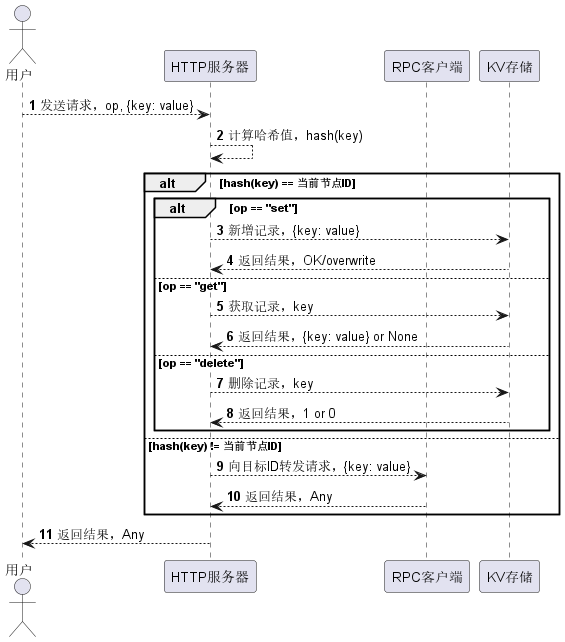
\includegraphics[width=0.8\linewidth]{examples/接收http流程.png}
    \caption{接收HTTP请求流程}
    \label{fig:recvhttp}
\end{figure}

图\ref{fig:recvhttp}描述了任一节点接收HTTP请求的详细流程。当用户向任意服务器节点发送HTTP请求后,该节点通过对键进行哈希函数获得唯一ID。如果ID与本地ID匹配,则与本地KV存储进行交互,通过操作字段op判断操作类型,之后选择对应的方法。如果ID与本地ID不匹配,则通过RPC客户端将请求转发给目标远程服务器。

接收RPC请求。

\begin{figure}[H]
    \centering
    \includegraphics[width=0.8\linewidth]{examples/接收RPC流程.png}
    \caption{接收RPC请求流程}
    \label{fig:recvrpc}
\end{figure}

图\ref{fig:recvhttp}描述了任一节点接收HTTP请求的详细流程。当RPC服务端收到来自任一节点的RPC客户端发送的RPC请求后,服务端所在节点就会通过操作字段op判断操作类型,并于本地KV存储交互,之后把请求返回给RPC客户端。

\subsubsection{接口描述}

本系统的接口描述如下。

\begin{table}[H]
    \centering
    \caption{接口描述}
    \label{tab:api}
    {
        \begin{tabularx}{0.9\linewidth}{|p{1cm}|p{1.1cm}|p{1.6cm}|p{1.8cm}|X|}
            \hline
            名称 & URL & 方法 & 请求参数 & 说明 \\
            \hline 
            新增 & / & POST & JSON & 上传格式为\{"key": "value"\}\newline 的JSON \\
            获取 & /\{key\} & GET & 键 & 当键存在时返回格式为\{"key": "value"\}的JSON,否则返回错误码404 \\
            删除 & /\{key\} & DELETE & 键 & 当键存在时返回1表示成功,否则返回0表示失败 \\
            \hline
        \end{tabularx}
    }
\end{table}

如表\ref{tab:api}所示,本系统的接口描述遵循Restful规范,通过POST/GET/DELETE等请求表示操作类型。